\section{Federkonstante}

\subsection{Arbeitsgrundlagen}

\subsection{Durchf\"uhrung}

\subsubsection*{Versuchsanordnung}

\subsubsection*{Messergebnisse}

\begin{center}
    \begin{threeparttable}
        \caption{Gemessene Gr\"ossen}
        \begin{tabular}{ccc}
            \toprule
            $F (N)$ & \hspace{12mm} & $z (m)$ \\
            \midrule
            3.83  & & 0.20 \\
            7.89  & & 0.35 \\
            8.08  & & 0.42 \\
            9.80  & & 0.46 \\
            10.58 & & 0.51 \\
            12.33 & & 0.54 \\
            12.23 & & 0.59 \\
            14.43 & & 0.67 \\
            15.51 & & 0.81 \\
            17.09 & & 0.80 \\
            \bottomrule
        \end{tabular}
        \begin{tablenotes}
            \small
            \item \textbf{Hinweis:} Daten wurden vom Auftragsdokument kopiert.
        \end{tablenotes}
    \end{threeparttable}
\end{center}

\[ \frac{\partial R}{\partial x} \biggr \rvert_{5}^{6} \]


\subsubsection*{QtiPlot}

\begin{figure}[H]
    \center
    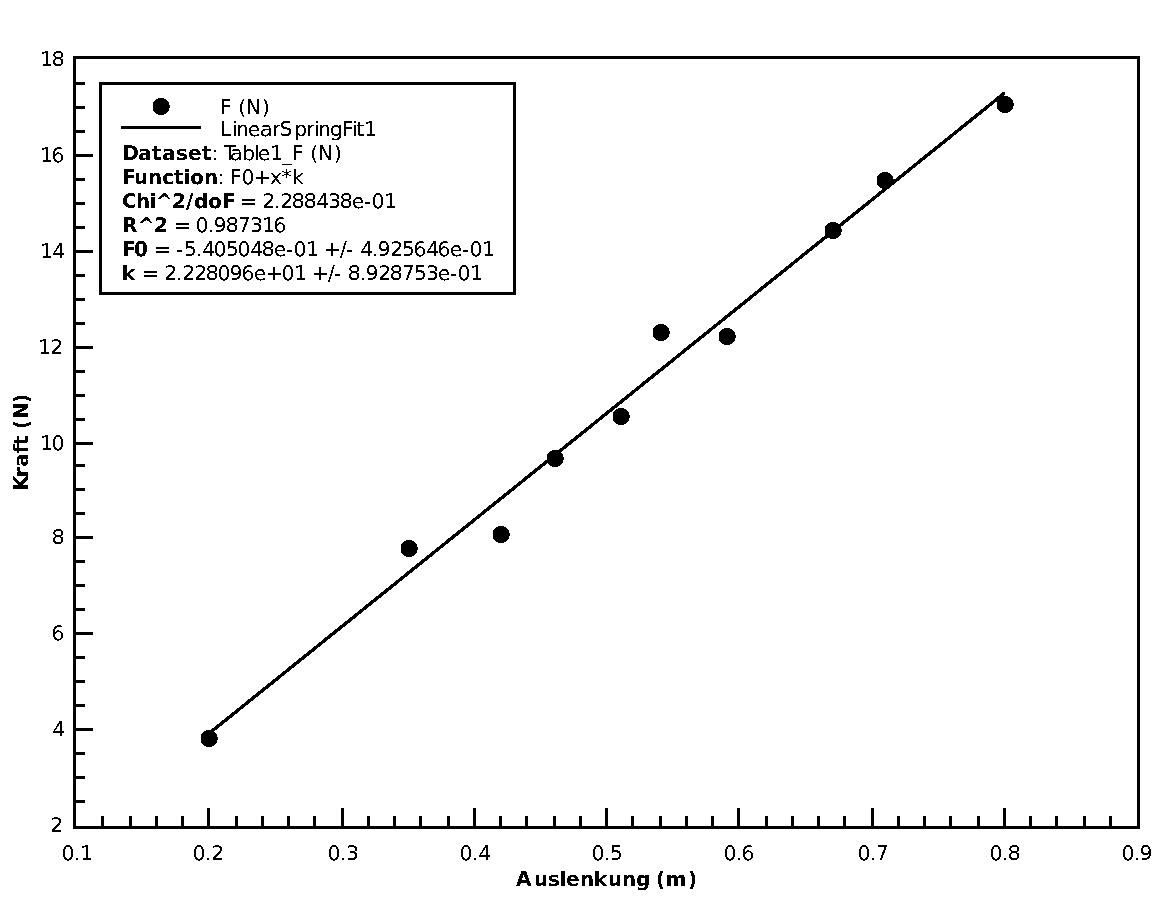
\includegraphics[width=.8\textwidth]{qtiplot/feder-linear}
    \caption{Lineare Regression zur Bestimmung von $k$ und $F_0$}
    \label{fig:feder-linear}
\end{figure}

\begin{figure}[H]
    \center
    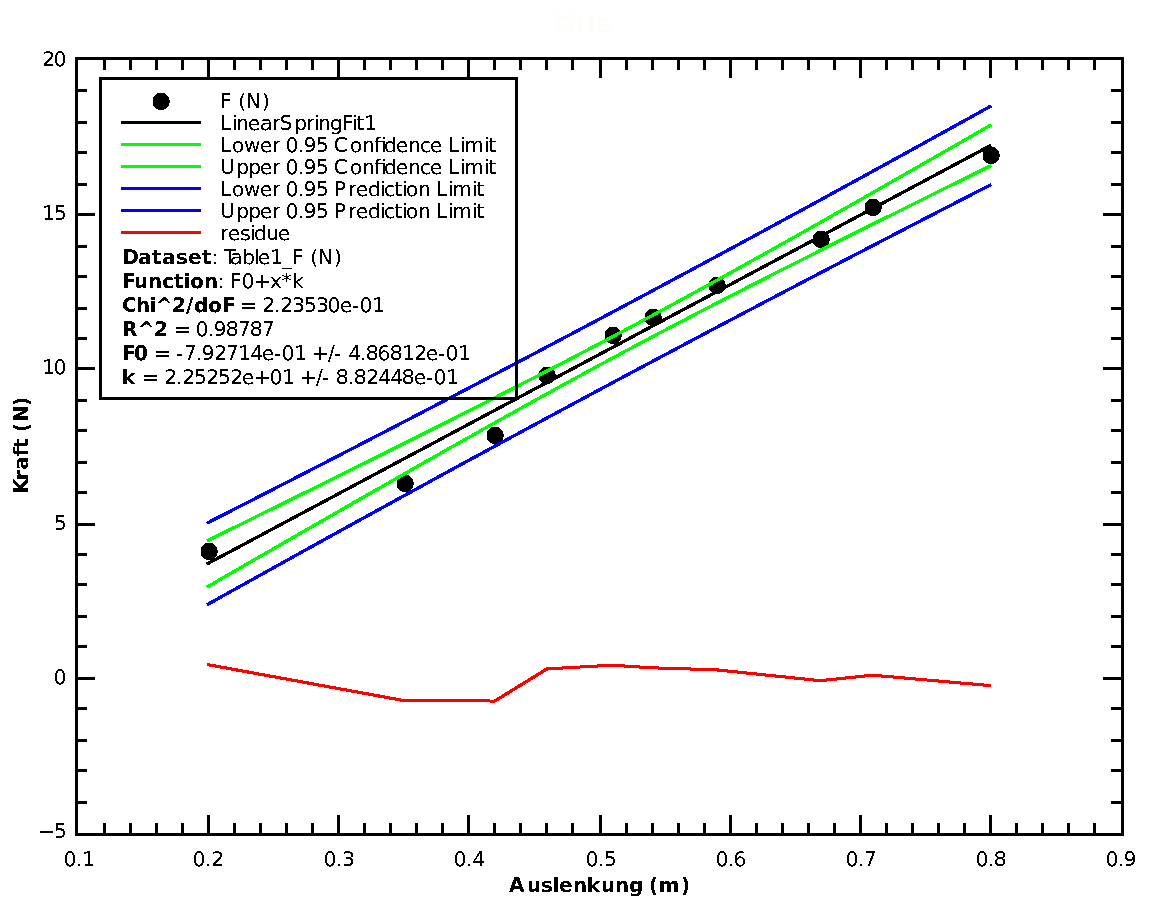
\includegraphics[width=.8\textwidth]{qtiplot/feder-95-bands}
    \caption{95\% Confidence- und Prediction-bands sowie Residuals}
    \label{fig:feder-95-bands}
\end{figure}

\begin{figure}[H]
    \center
    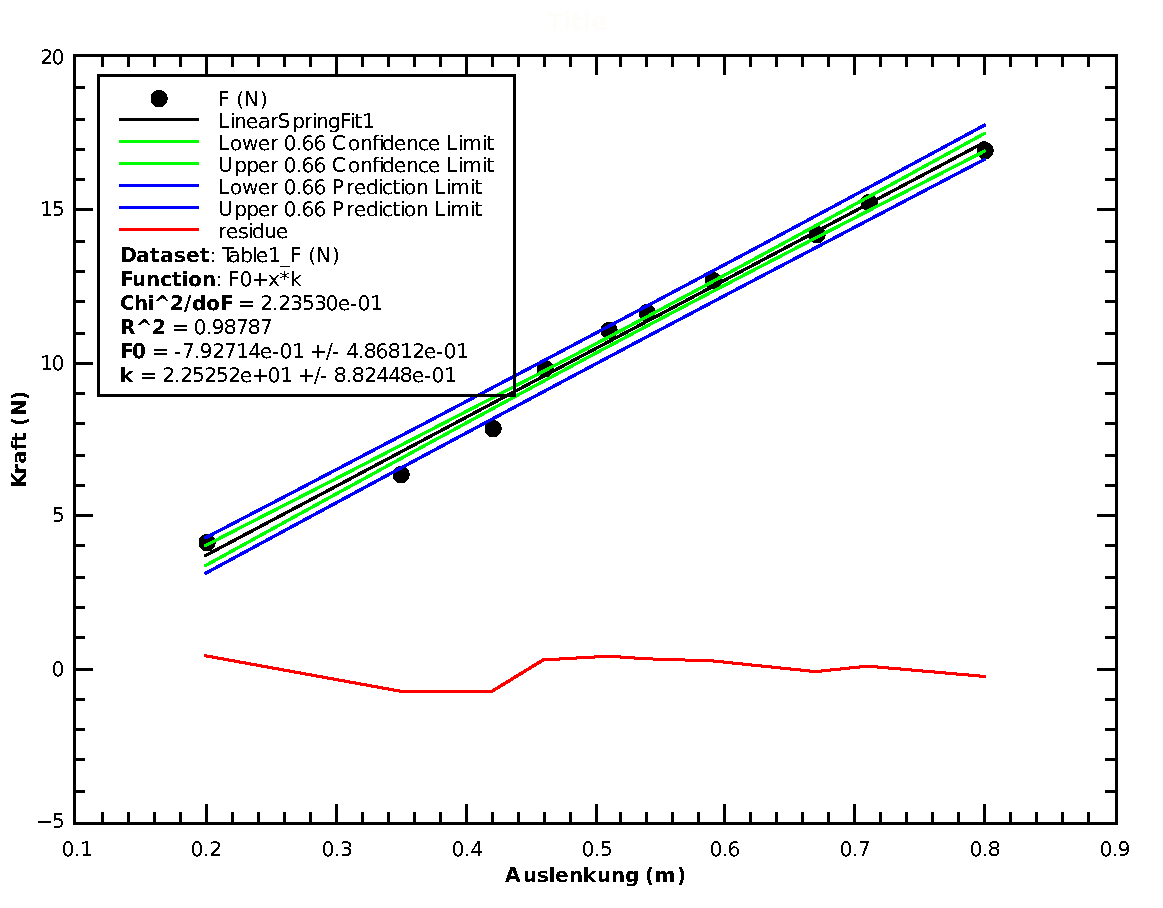
\includegraphics[width=.8\textwidth]{qtiplot/feder-66-bands}
    \caption{66\% Confidence- und Prediction-bands sowie Residuals}
    \label{fig:feder-66-bands}
\end{figure}

